% --------------------------------------------------------------------
% Beamer Template 
% --------------------------------------------------------------------
% Necessary infos for documentstyle
\documentclass[compress]{beamer}

\usetheme{Stud}
\usepackage{times}
\usepackage[utf8]{inputenc}
\usepackage[T1]{fontenc} % nicht benoetigt, in folien wird eh nicht getrennt
\usepackage{ngerman}
\usepackage{graphicx}
%\usepackage{color}% color wird bereits von beamer geladen
\usepackage{verbatim}
\usepackage{psfrag}
\usepackage{math}
\usepackage{calc}
\usepackage{tabularx}
\usepackage{enumerate}
\usepackage{algorithm,algorithmic}
\usepackage{pifont}
\usepackage{upgreek}



% --------------------------- Helpers ----------------------------
% to use these texts in two languages
% changes the parameter within {#}
% 1 = German
% 2 = English
\def\twolang#1#2{#2} 
\let\2=\twolang

% --------------------------------------------------------------------


\bibliographystyle{ieeetr}
\setbeamertemplate{bibliography item}{\insertbiblabel}

\graphicspath{{images/}}


% --------------------------------------------------------------------
\title{Reactive Construction Of Planar, Euclidean t-Spanners With Constant Node Degree}
\subtitle{Antrittsvortrag zur Bachelorarbeit}
\author[T. Budweg]{Tim Budweg}
\institute{
  \texttt{tbudweg@uni-koblenz.de} \\
  \vspace{0.2cm}
  \2{AG Rechnernetze\\
  Universität Koblenz-Landau}{Institute for Computer Science\\
  University of Koblenz-Landau}
}
\date{February 10th, 2016}
% --------------------------------------------------------------------



% document
\begin{document}
\frame{\titlepage}

%\logo{...} erst hier, damit es nicht mit auf die Titelseite kommt!
%\logo{\pgfuseimage{logo}}

%\part{Overview}
%\section{\2{Überblick}{Overview}}
%\frame{
%  \frametitle{\2{Überblick}{Overview}}
%  \tableofcontents[part=2,hideallsubsections]
%}

% ====================================================================
% ====================================================================

% here comes the real content which is part of scontent.tex
\part{Content}

% ---------------------------------------------------------------------------
% - For showing graphics and text on one slide use:
%   \begin{columns}[T]
%	\begin{column}[T]{.5\linewidth}
%	    \includegraphics[width=\linewidth]{<filename>}
%	\end{column}
%	\begin{column}[T]{.5\linewidth}
%	    <content>
%	\end{column}
%   \end{columns}
% ---------------------------------------------------------------------------

%\begin{frame}
%\frametitle{}
%\begin{itemize}
%
%\end{itemize}
%\end{frame}

\subsection{Introduction}
%\begin{frame}
%\begin{itemize}
%\item Was ich gemacht habe
%\item erklärungen reactive, planar, t-spanner, constant node degree
%\item motivation warum ich das gemacht habe
%\end{itemize}
%\end{frame}

\begin{frame}
\frametitle{Goal}
Algorithm which satisfies the following graph-properties:
\begin{itemize}
\item planar
\item Euclidean t-spanner
\item constant node degree
\item constructed in a reactive way (beaconless, without any prior neighborhood information)
\end{itemize}
\end{frame}

\begin{frame}
\frametitle{Motivation}
Use case: large, static ad-hoc networks (e.g. caution for tsunamis or fire in large areas)
\begin{itemize}
\item reactive: saves a lot of messages
\item constant node degree: only constant number of node addresses has to be stored
\item theoretical aspect: more properties may lead to possibly better results and graphs
\end{itemize}
\end{frame}

\subsection{Algorithm}
%\begin{frame}
%\begin{itemize}
%\item wie der algorithmus läuft
%\item rPDT
%\item MYS
%\item RMYS
%\end{itemize}
%\end{frame}

\begin{frame} 
\frametitle{rPDT \footcite{pdt, Neumann2012}}
	\begin{itemize}
    \begin{columns}[T]
	\begin{column}[T]{.3\linewidth}
    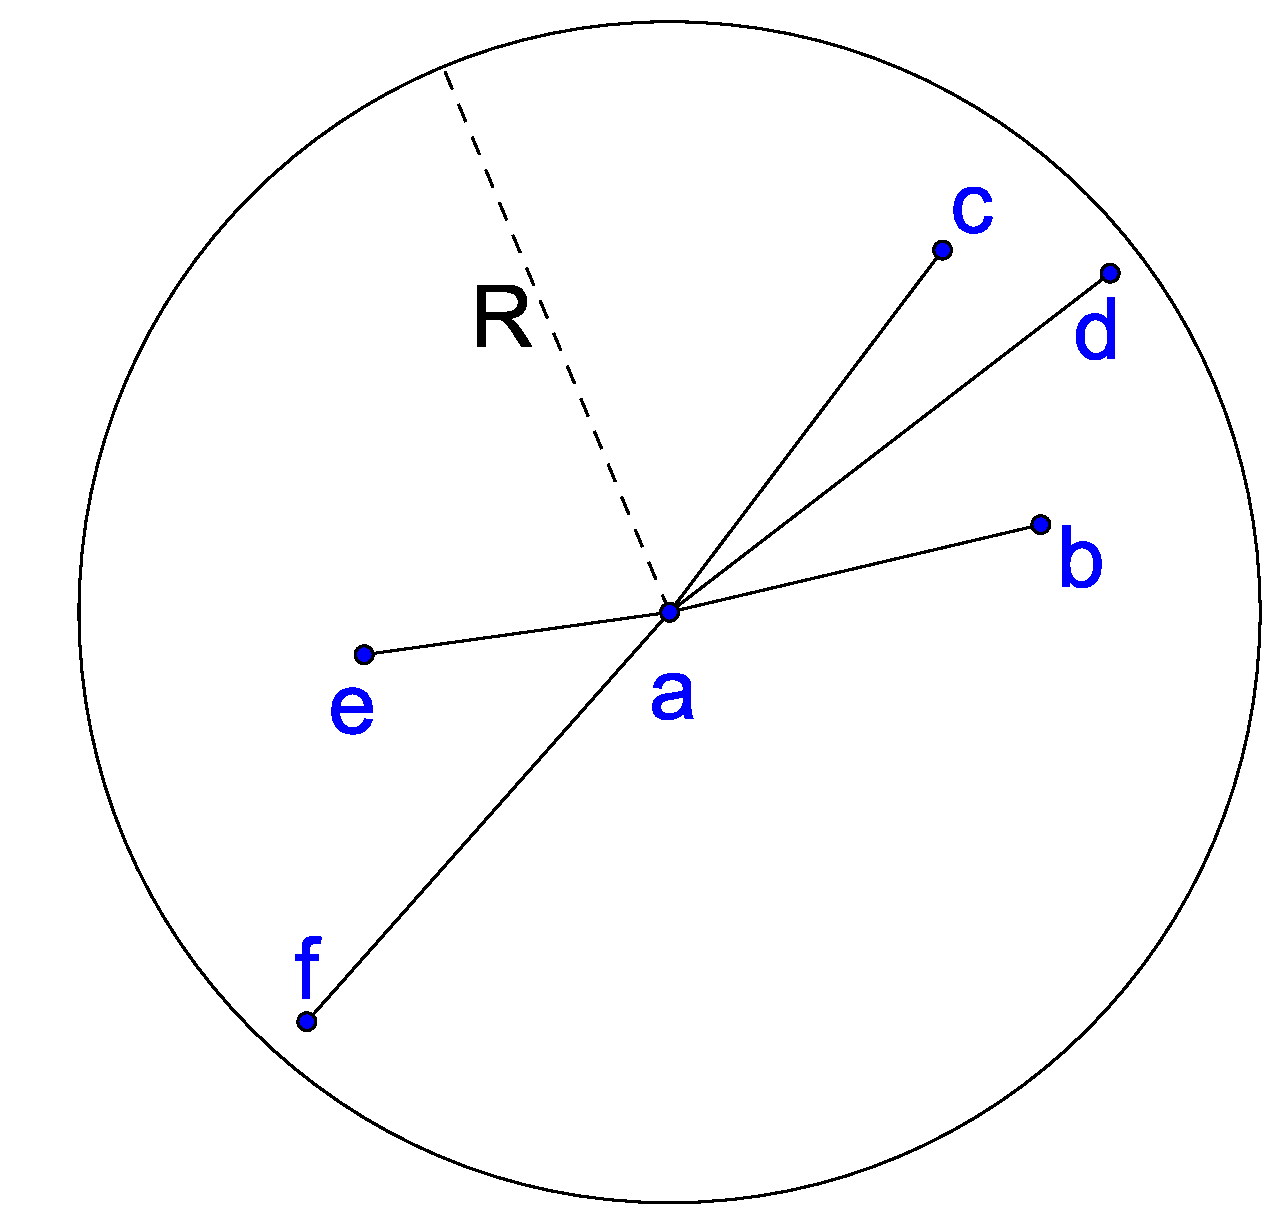
\includegraphics[width=\linewidth]{PDT_1.eps}
	\end{column}
	\begin{column}[T]{.7\linewidth}
	\item $a $ broadcasts start.
	\item All other nodes create timer.
	\item As soon as a timer stops related node sends a message to $a $, if a geometric condition is still satisfied.
	\end{column}
   \end{columns}
	\end{itemize}
\end{frame}

%geometric condition: circles -> Gabriel circle or PDT-circles with 
\begin{frame} 
\frametitle{rPDT}
\center 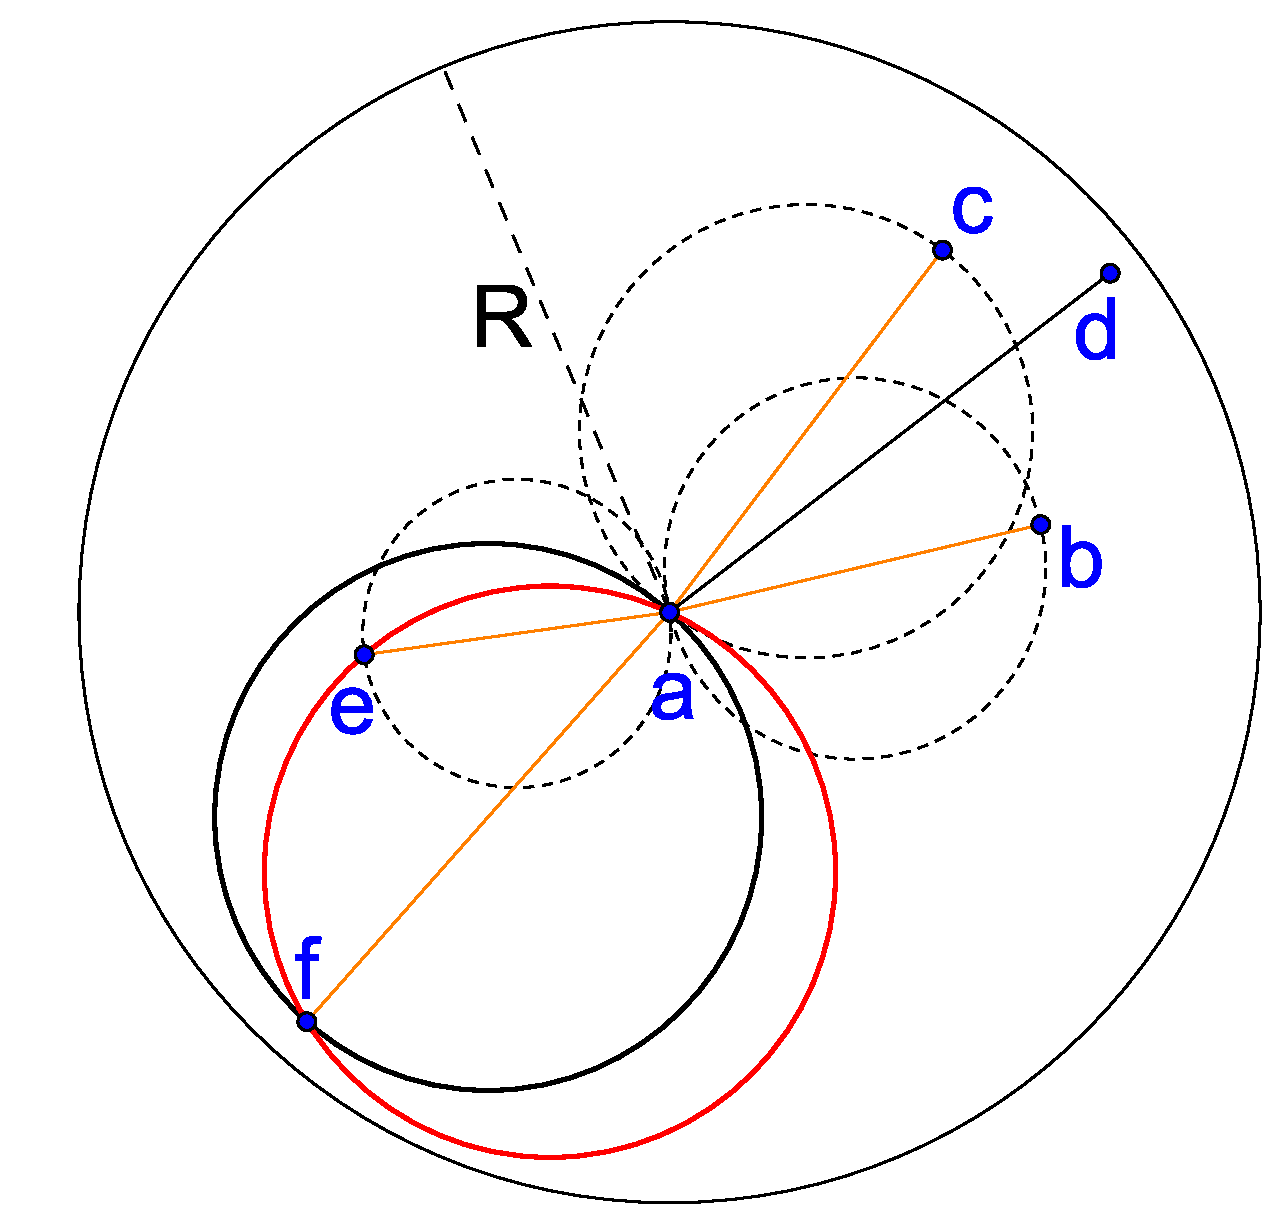
\includegraphics[width=0.7\linewidth]{PDT_3.eps}
\end{frame}

\begin{frame}
\frametitle{rPDT}
\center 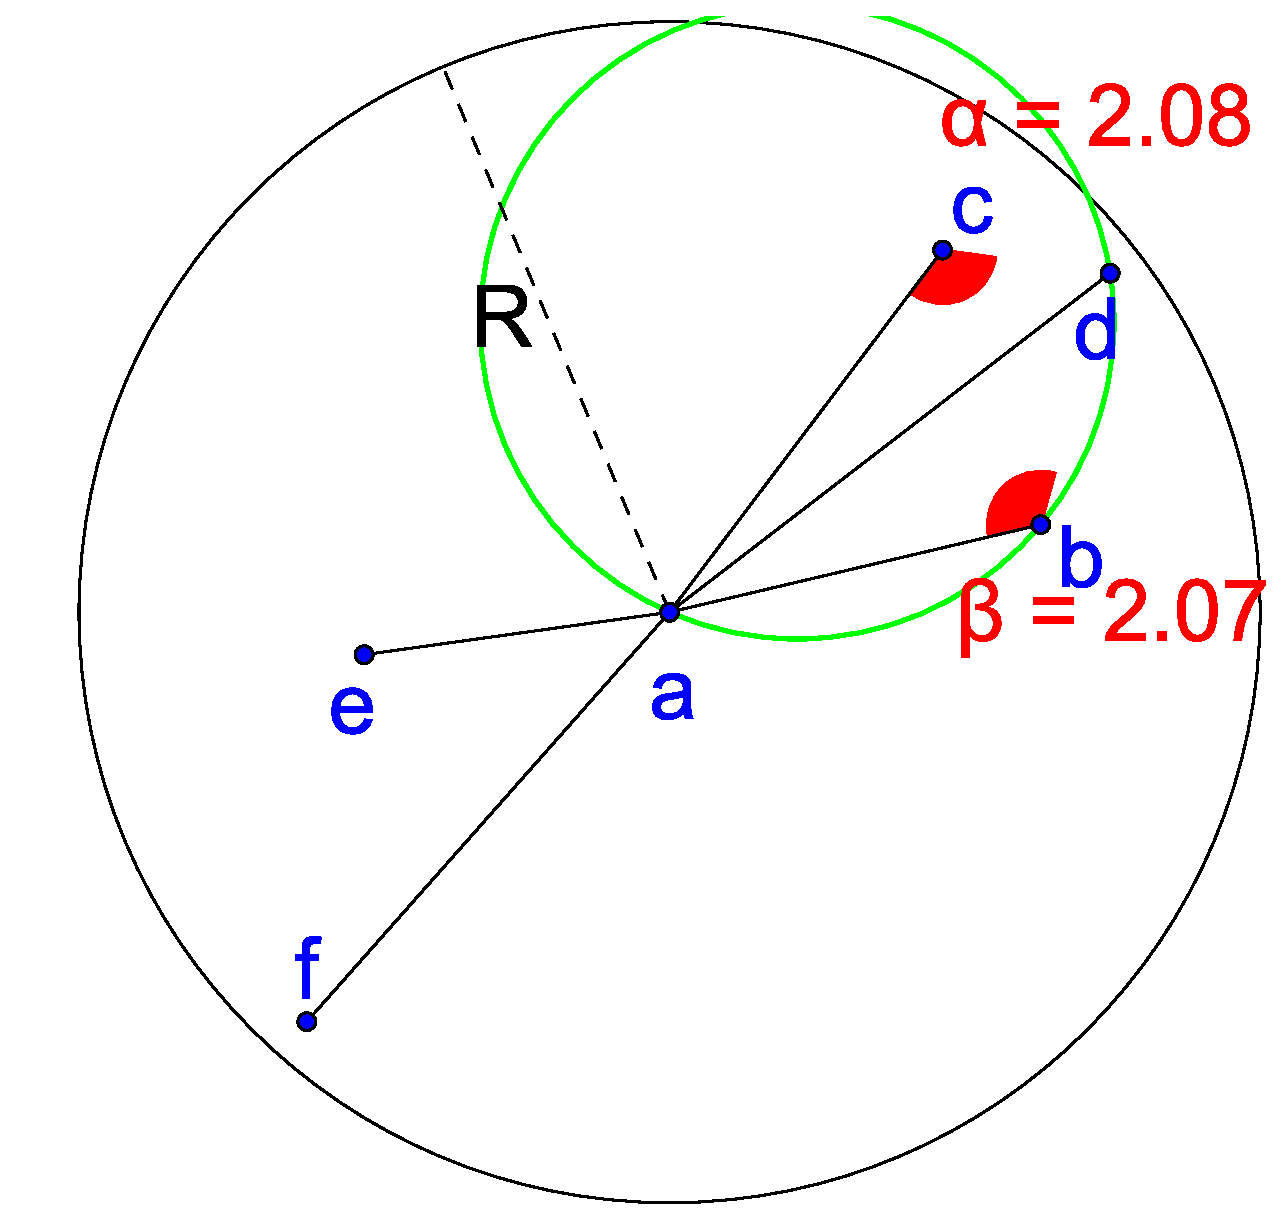
\includegraphics[width=0.7\linewidth]{PDT_angle.eps}
\end{frame}

%MYS
\begin{frame}
\frametitle{Modified Yao Step \cite{kanj}}
Input: planar, t-spanner (PDT)\\
Output: constand node degree of $k = 14 $
	\begin{enumerate}
		\item create $k $ equal cones
		\item for each non-empty cone find shortest edge
		\item for every empty cone try to find another edge according to sequence rules
		\item check, whether both endpoints of an edge have selected this edge
	\end{enumerate}
\end{frame}

\begin{frame} 
\frametitle{MYS}
	\center 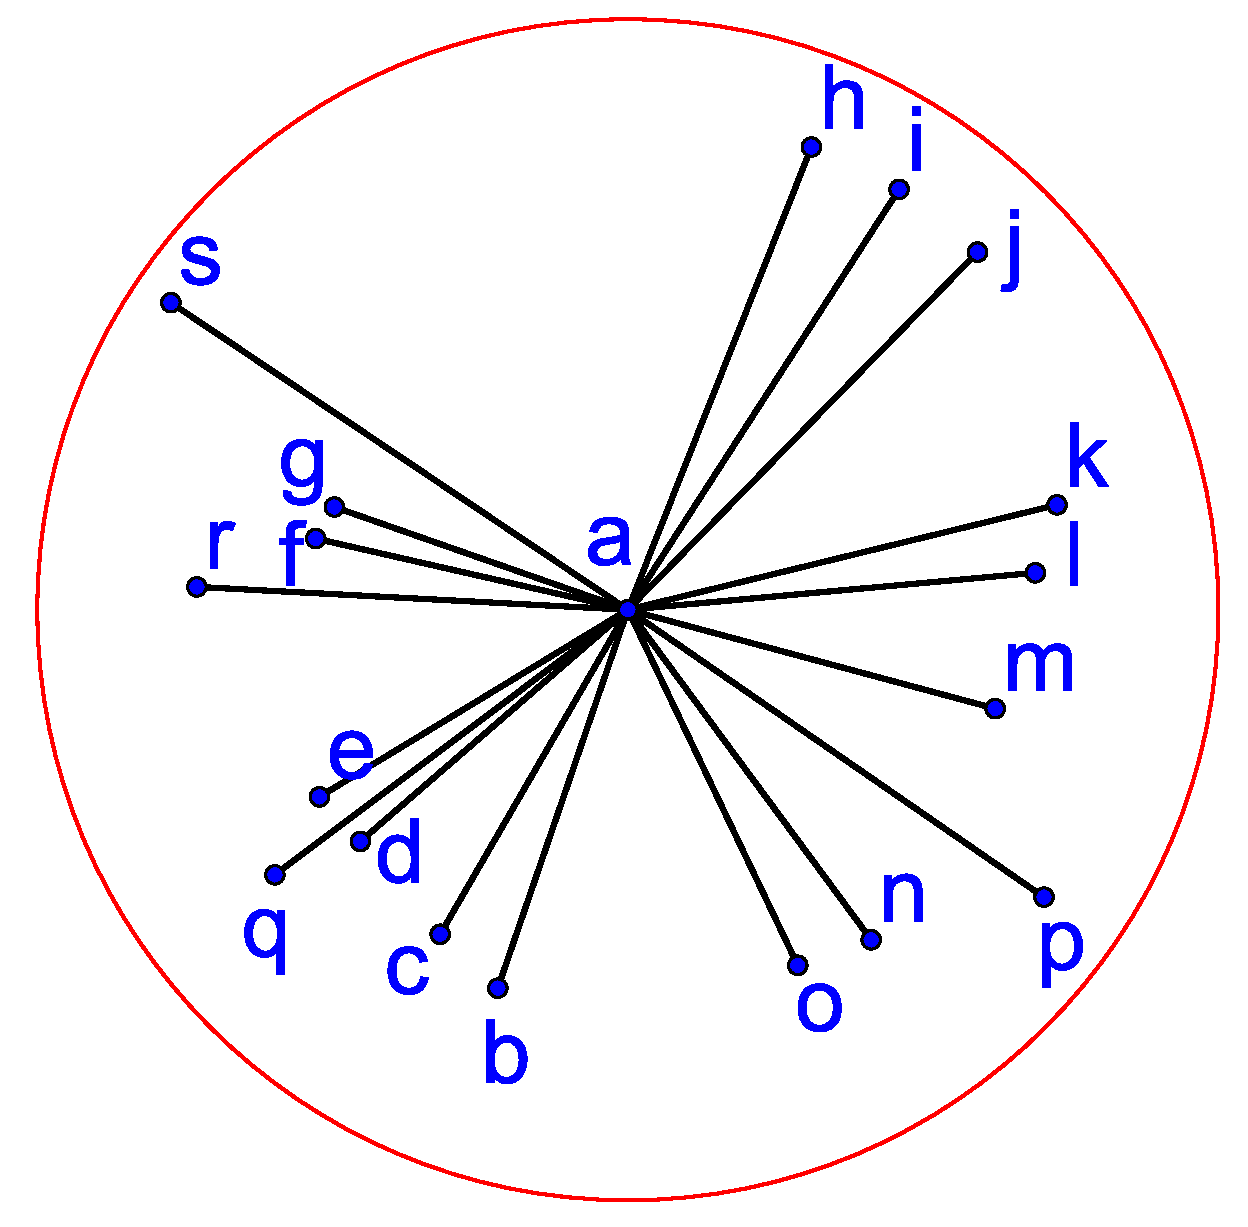
\includegraphics[width=0.65\linewidth]{RMYS_0.eps}
\end{frame}

\begin{frame} 
\frametitle{MYS - Step 1/3}
	\center 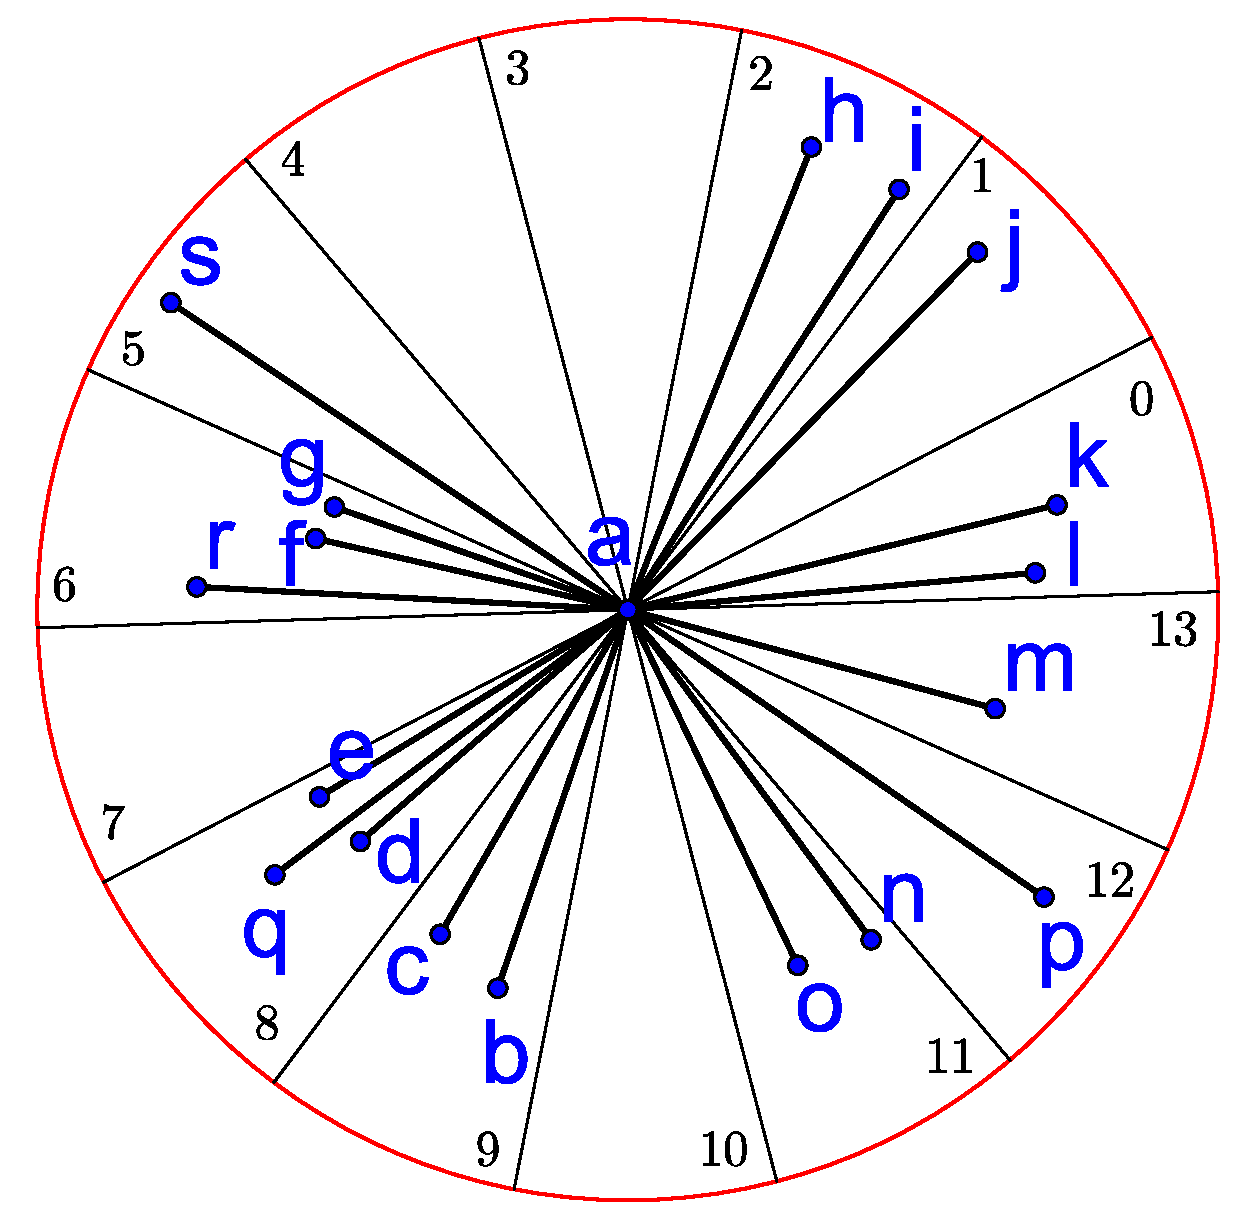
\includegraphics[width=0.65\linewidth]{RMYS_1.eps}
\end{frame}

\begin{frame} 
\frametitle{MYS - Step 2/3}
	\center 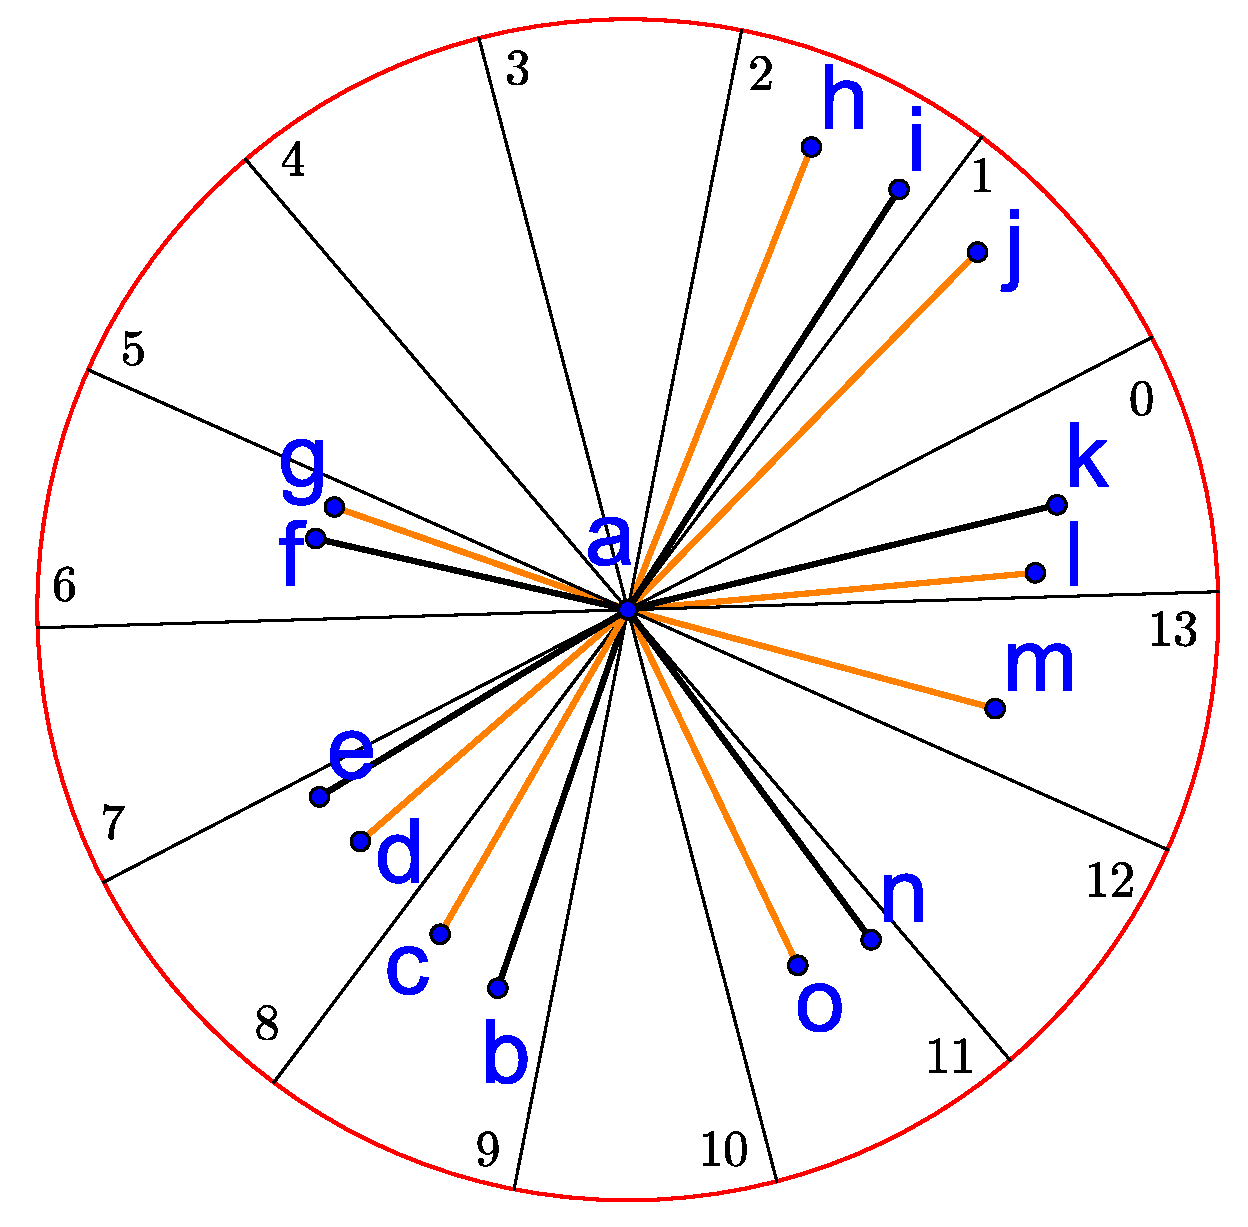
\includegraphics[width=0.65\linewidth]{RMYS_2.eps}
\end{frame}

\begin{frame} 
\frametitle{MYS - Step 3/3}
	\center 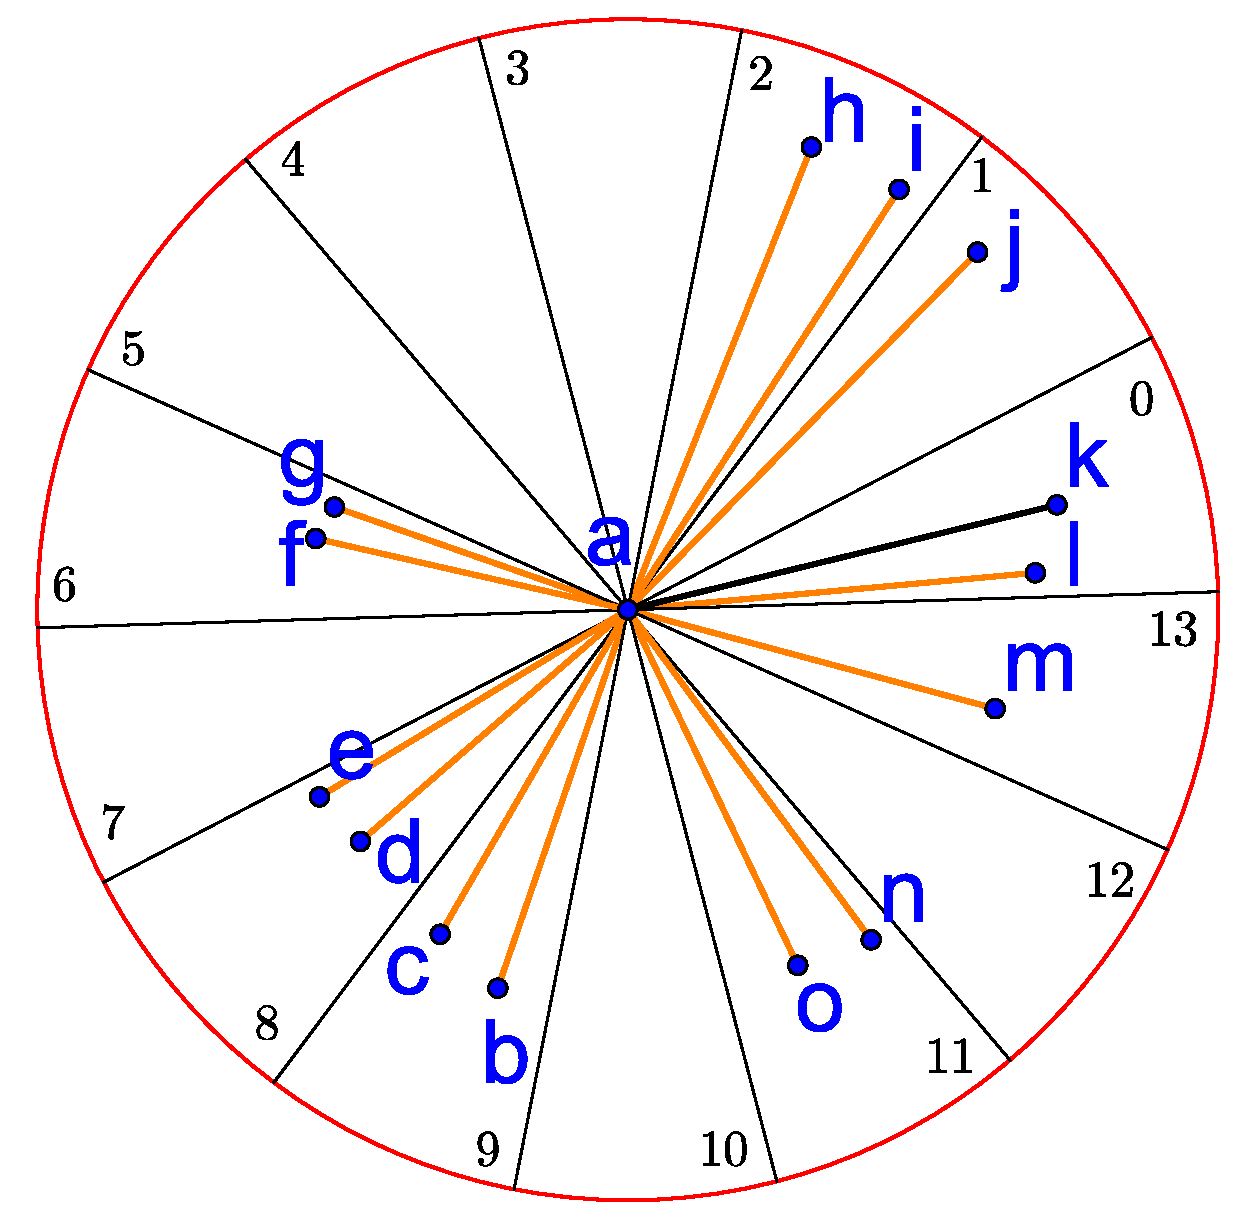
\includegraphics[width=0.65\linewidth]{RMYS_3.eps}
\end{frame}

\begin{frame}
\begin{algorithm}[H]
\begin{algorithmic}[0]
\STATE \textbf{Input:} any connected graph $G $; integer $k\geq 14 $
\STATE \textbf{Output:} planar, connected graph $G' $ with constant node degree of at most $k $
\FOR{each node $p \in G $}
\STATE create the PDT-Neighborhood of $p $ using rPDT
\STATE apply rMYS to $p $ using PDT-graph
\STATE let each neighbor of $p $ create its RMYS neighbors and send a protest message if $p $ is not among them causing $p $ to remove this edge
\ENDFOR
\end{algorithmic}
\caption{RMYS}
\end{algorithm}
\end{frame}


\subsection{Results}
%\begin{frame}
%\begin{itemize}
%\item Plots und Erklärung dazu
%\item Eigenschaften zeigen
%\item Warum formaler Beweis für Spanner nicht geklappt hat.
%\end{itemize}
%\end{frame}

\begin{frame} 
\frametitle{Average neighbors}
\center	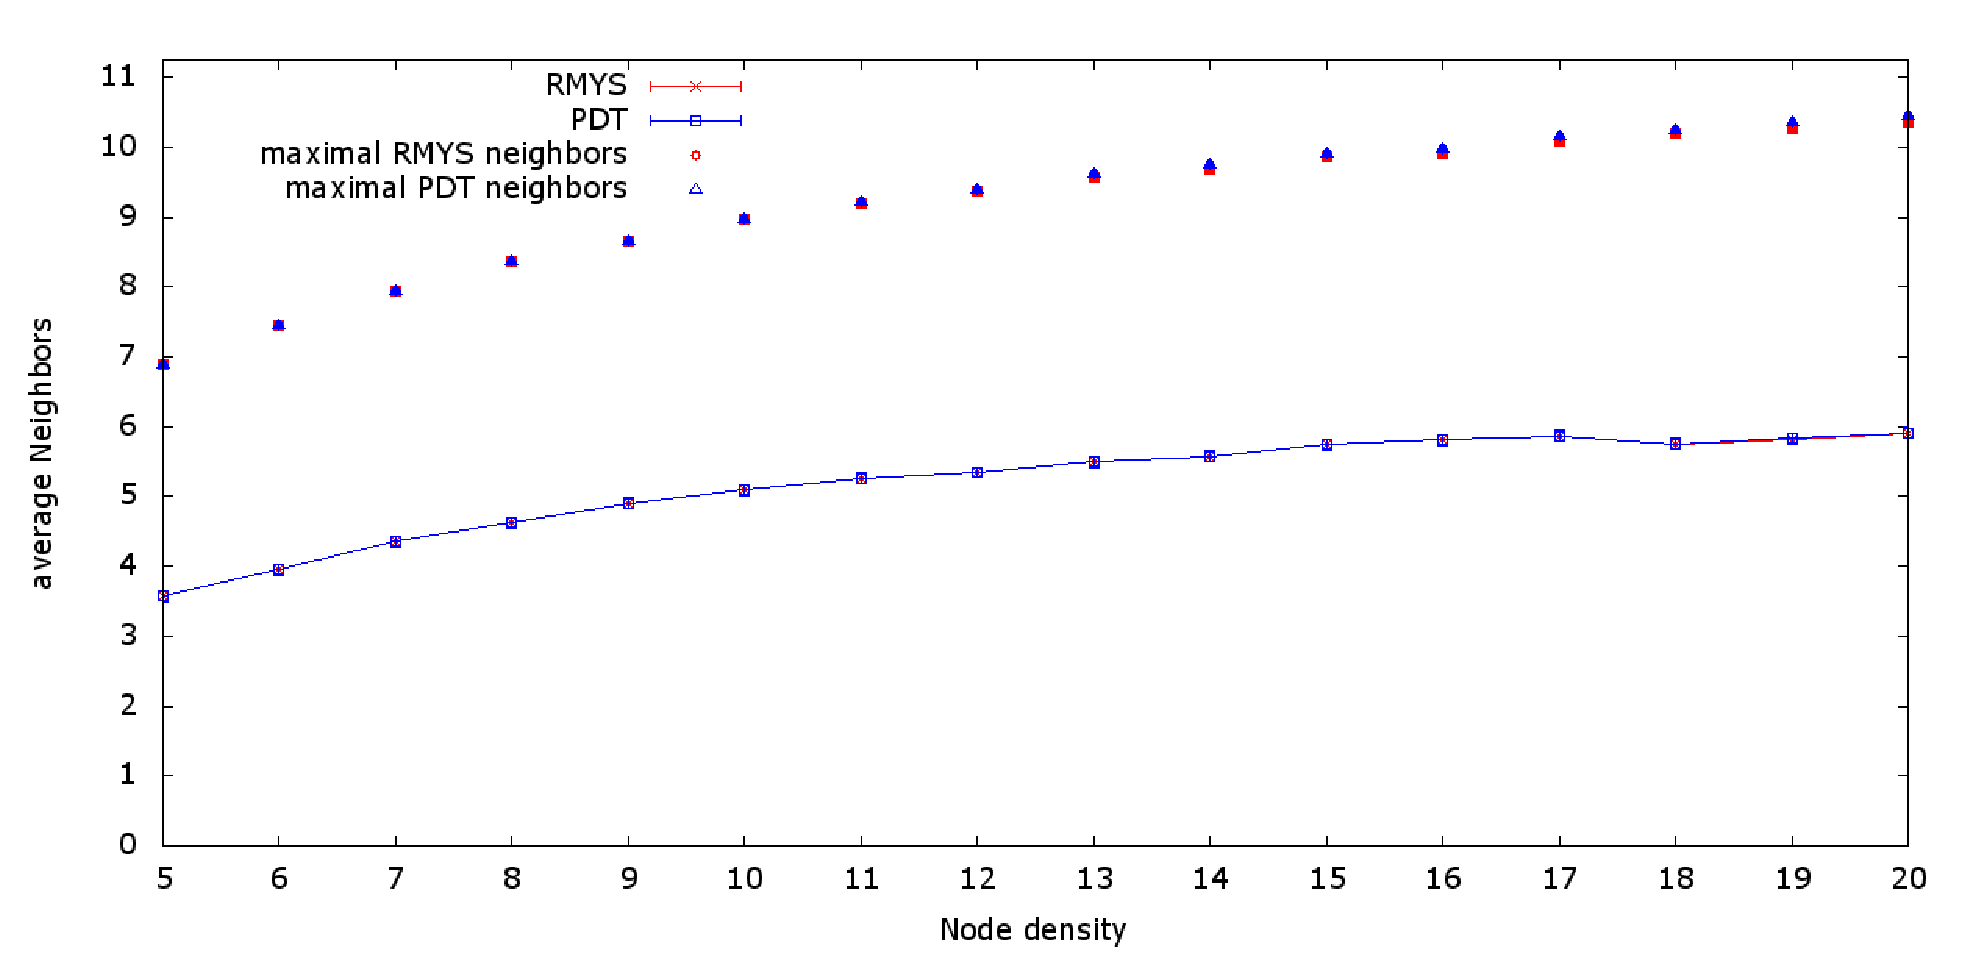
\includegraphics[width=1.0\linewidth]{RMYS_PDT_avrNeighbors.eps}
\end{frame}

\begin{frame} 
\frametitle{Euclidean spanning-ratio}
\center	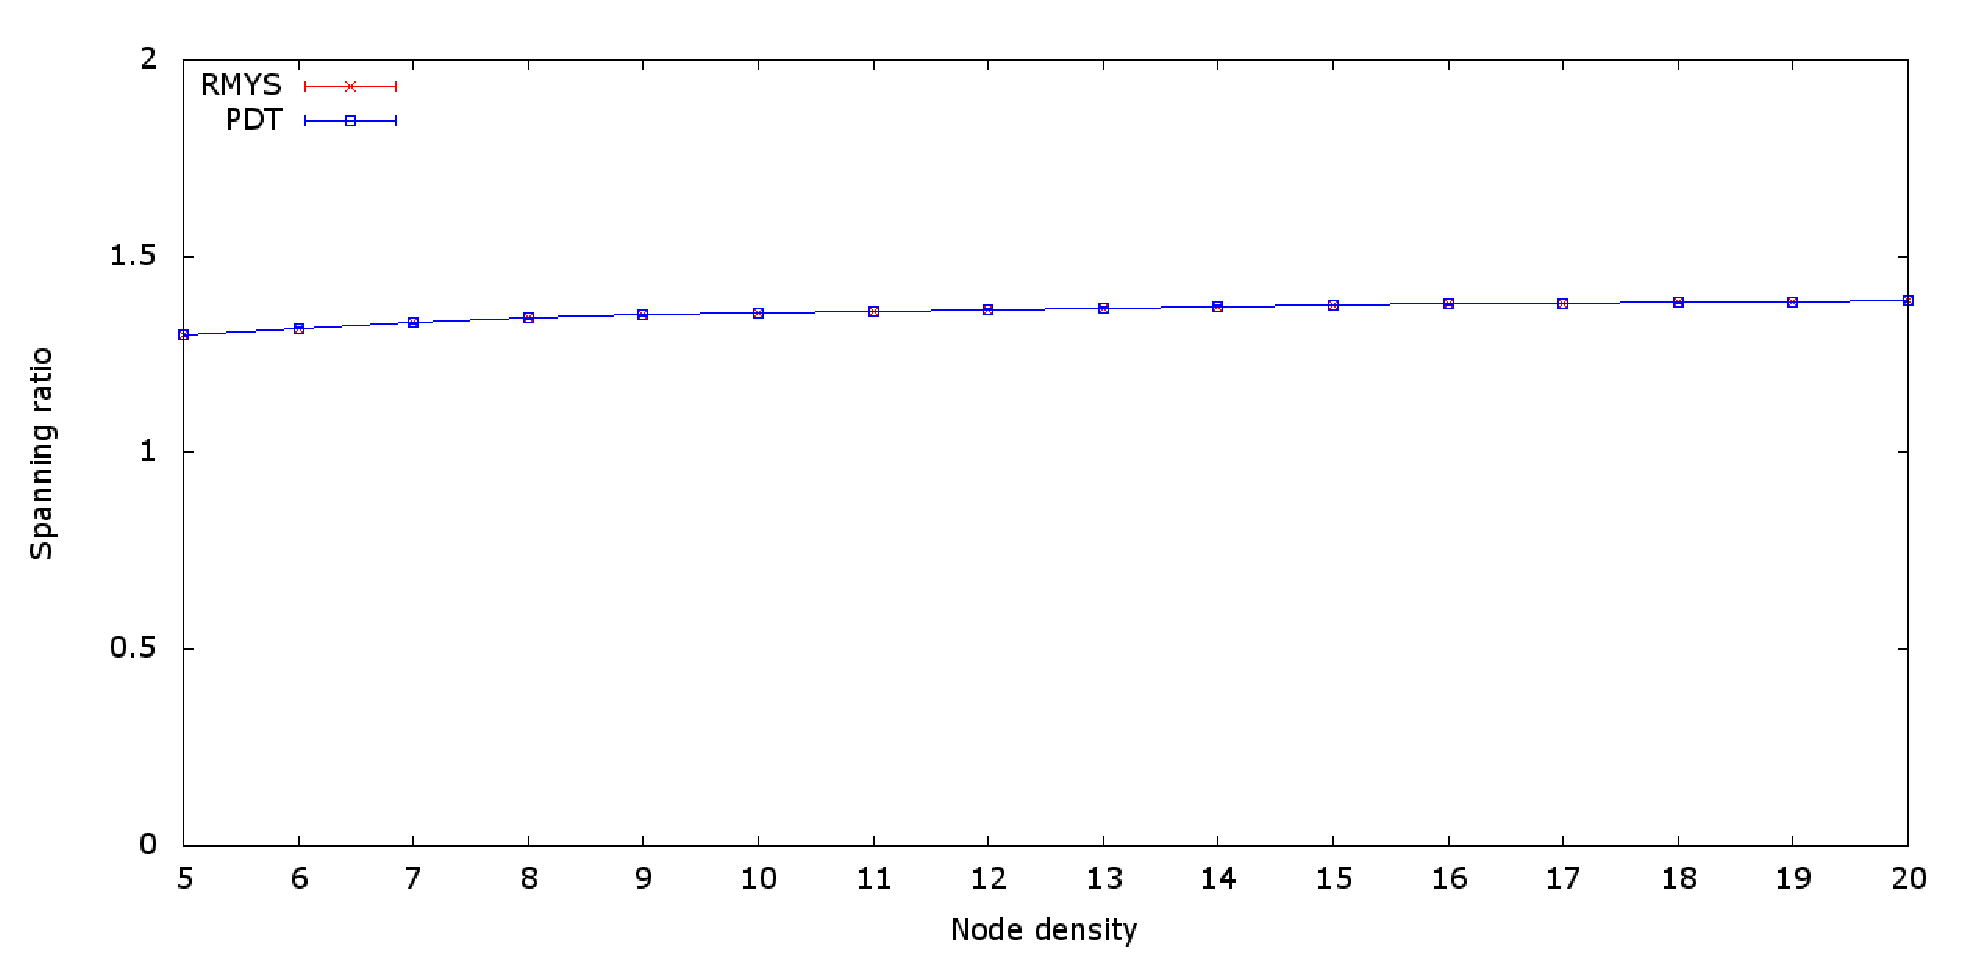
\includegraphics[width=1.0\linewidth]{RMYS_PDT_SpanningRatio.eps}
\end{frame}

\begin{frame} 
\frametitle{Euclidean spanning-ratio}
\center	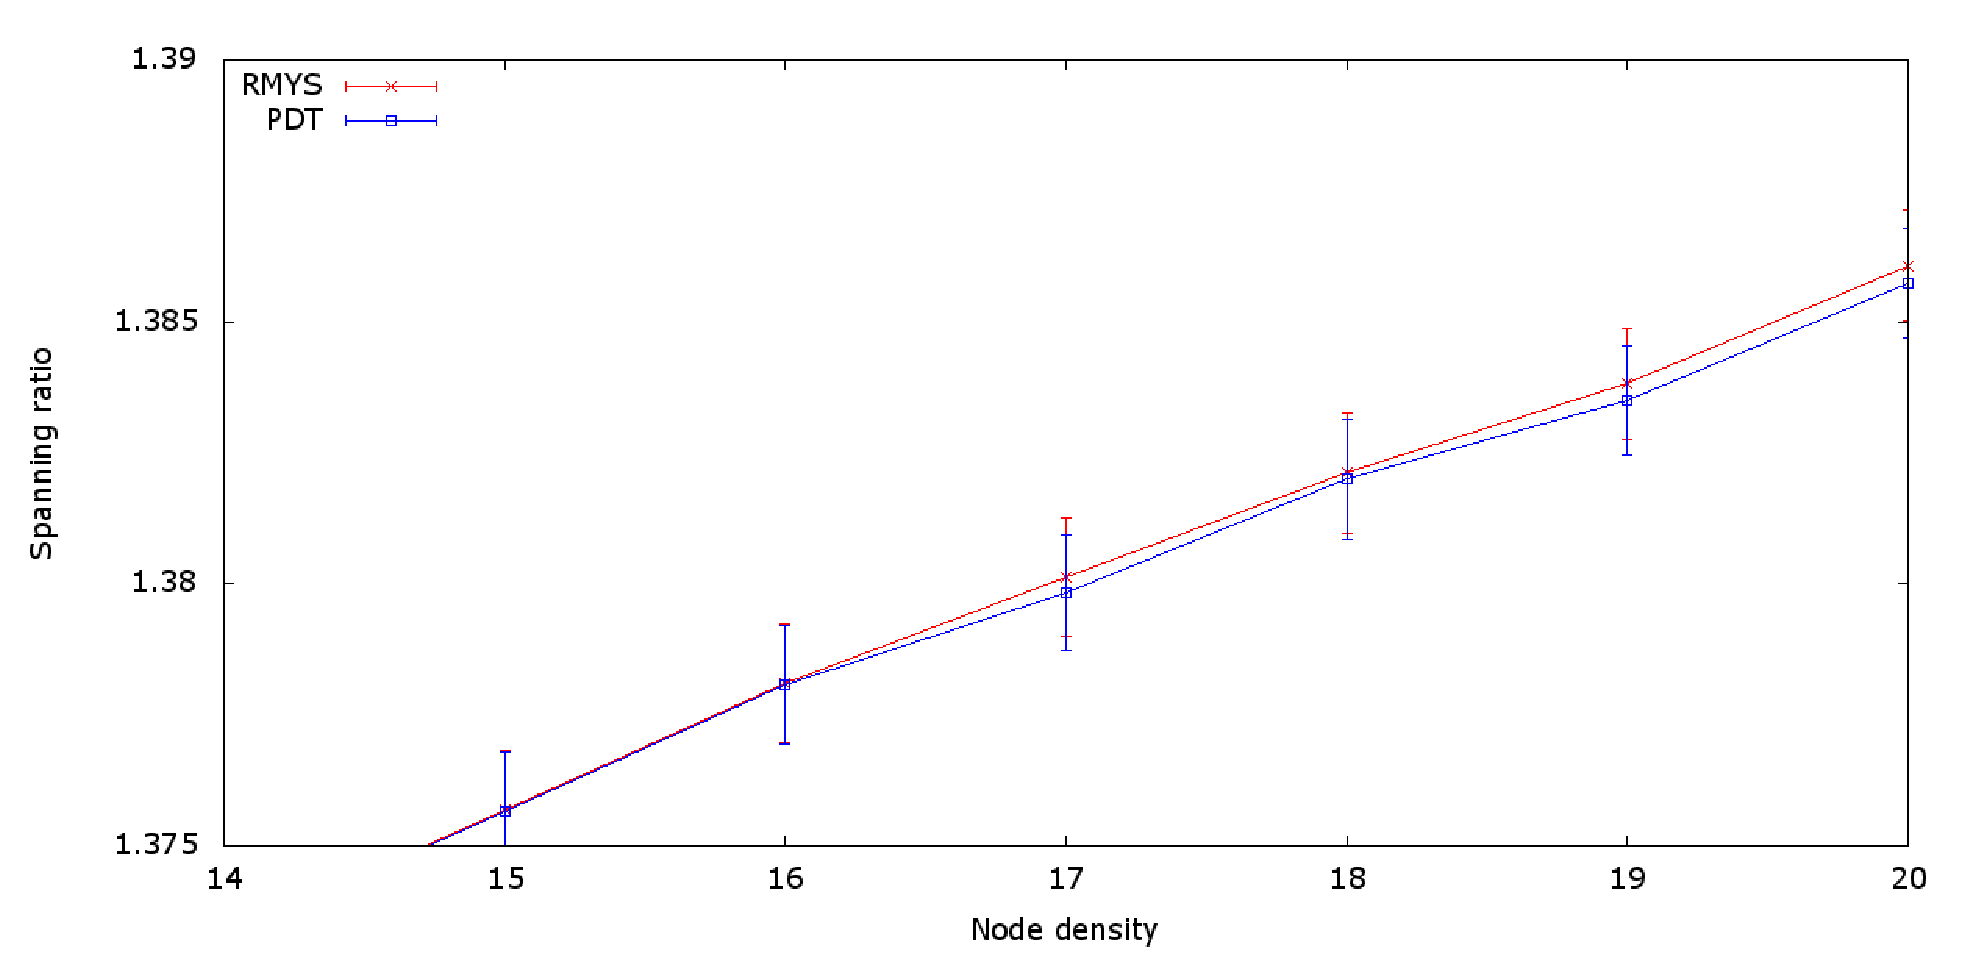
\includegraphics[width=1.0\linewidth]{RMYS_PDT_SpanningRatio-hd.eps}
\end{frame}

\begin{frame} 
\frametitle{Hop spanning-ratio}
\center	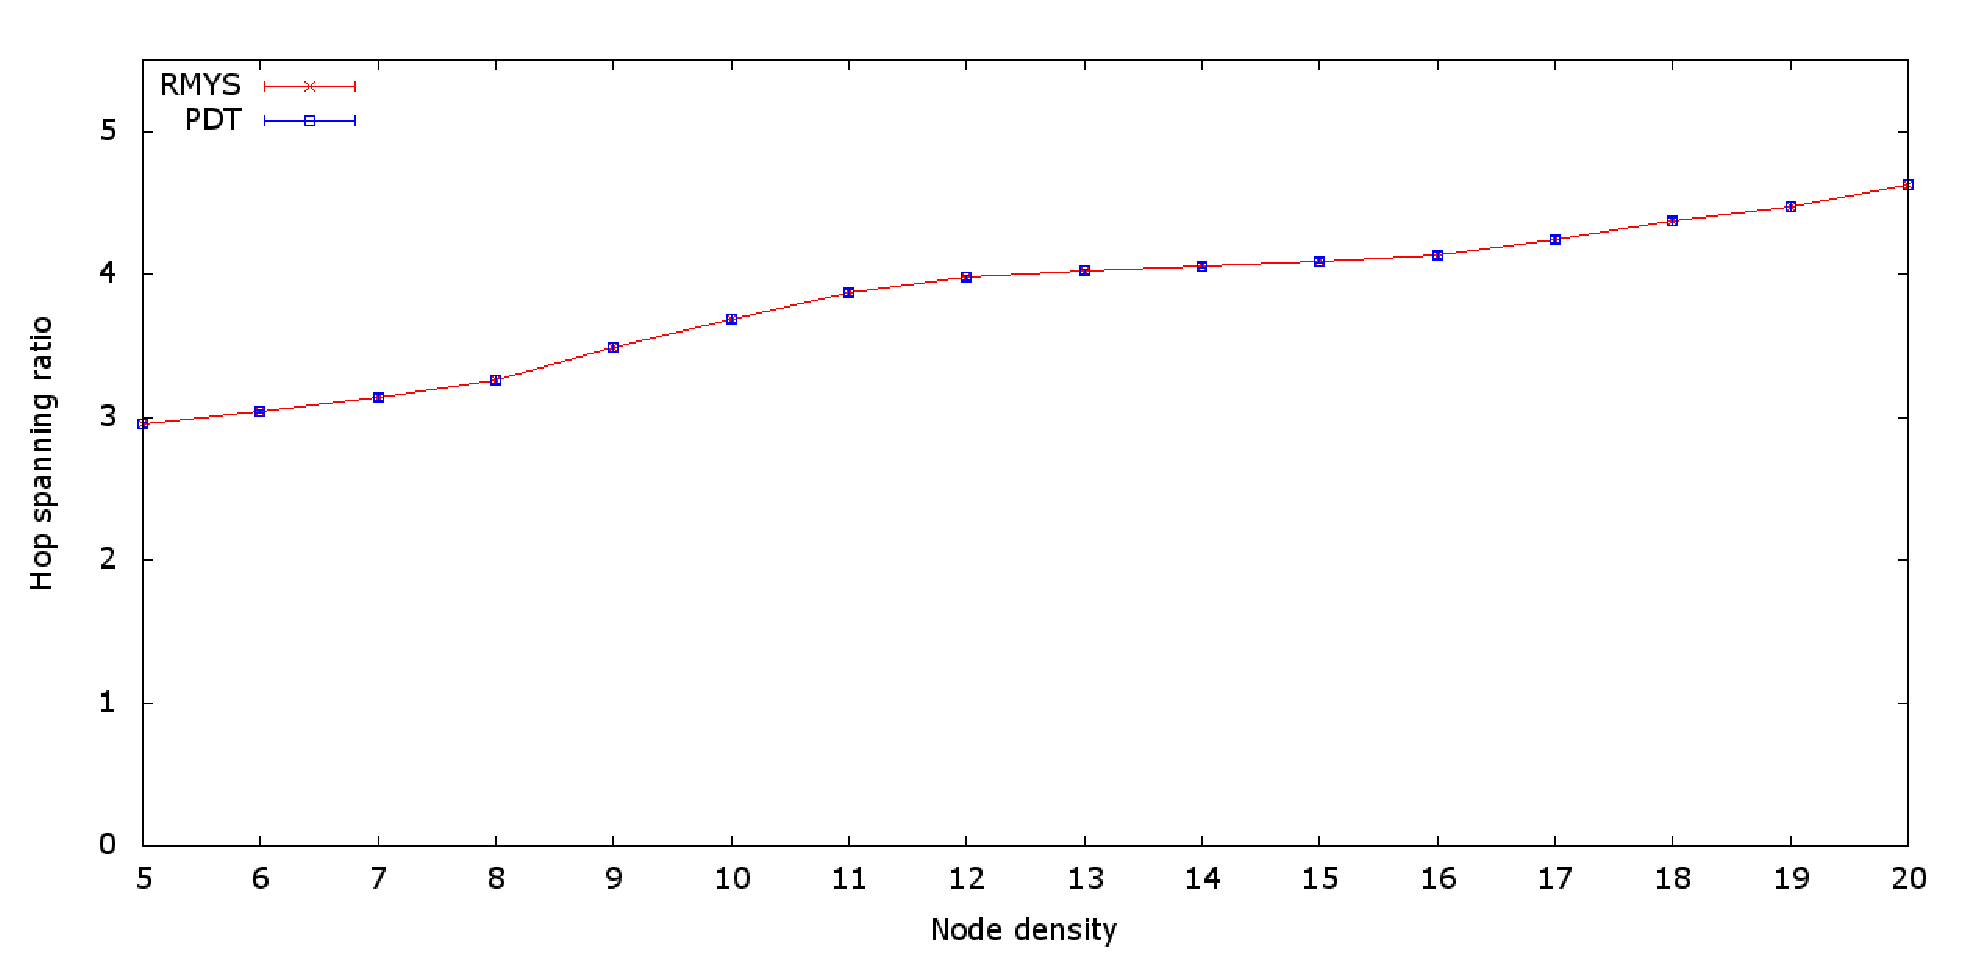
\includegraphics[width=1.0\linewidth]{RMYS_PDT_HopSpanningRatio.eps}
\end{frame}


\begin{frame} 
\frametitle{Number of messages with respect to node density}
\center	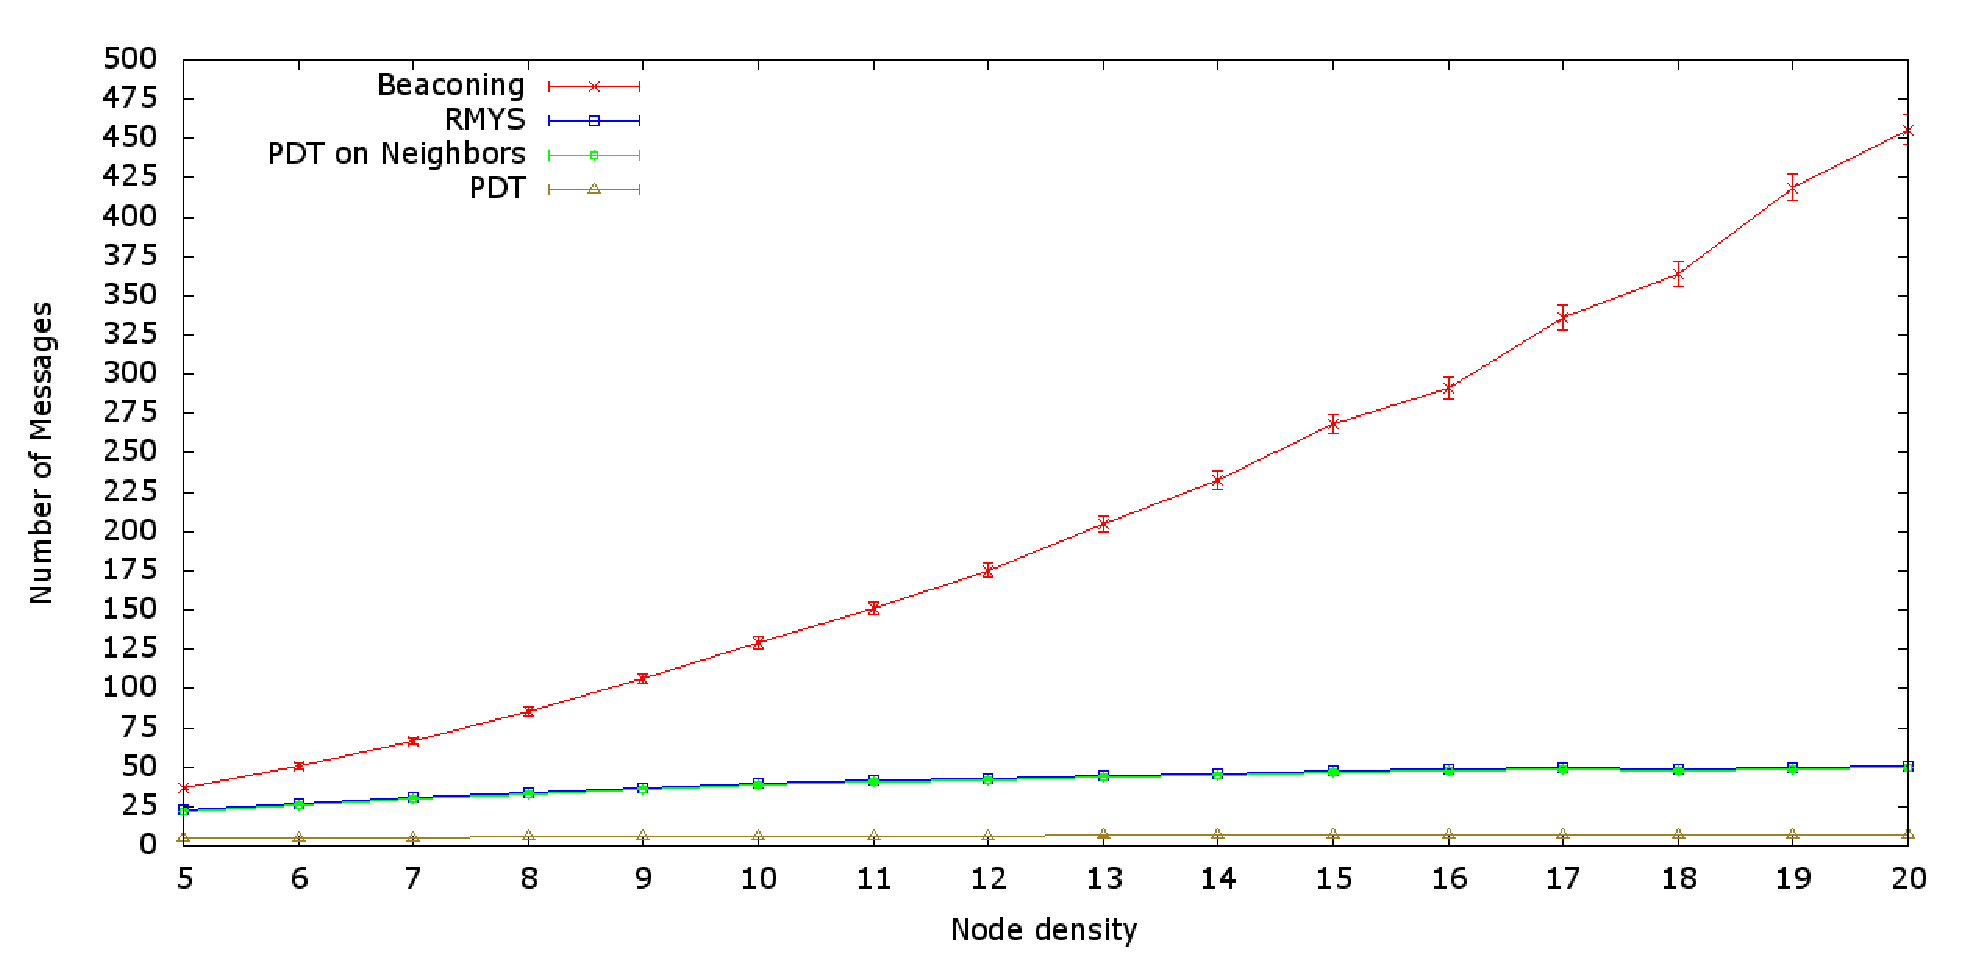
\includegraphics[width=1.0\linewidth]{RMYS_PDT_Beaconing_Neighbors.eps}
\end{frame}

\begin{frame} 
\frametitle{Number of messages with respect to node density}
\center	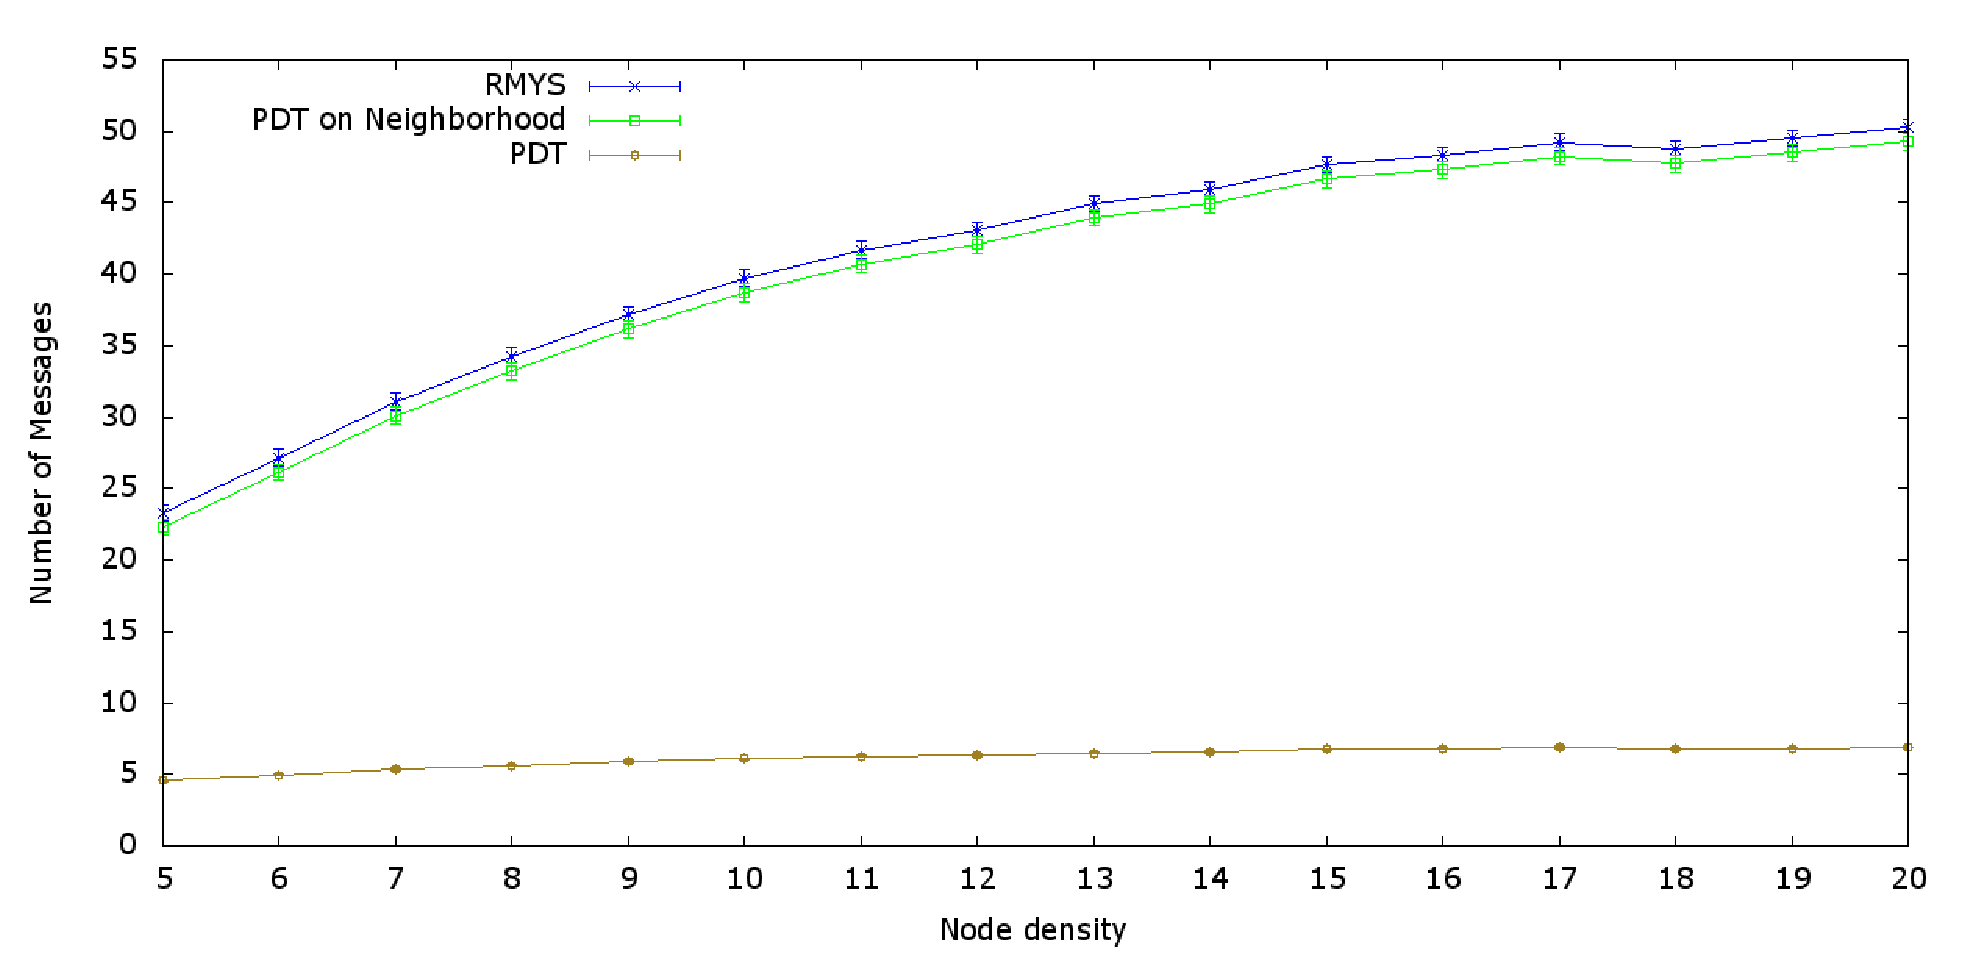
\includegraphics[width=1.0\linewidth]{RMYS_PDT_Neighbors.eps}
\end{frame}

\begin{frame} 
\frametitle{Neighbors per UDG-neighbors}
\center	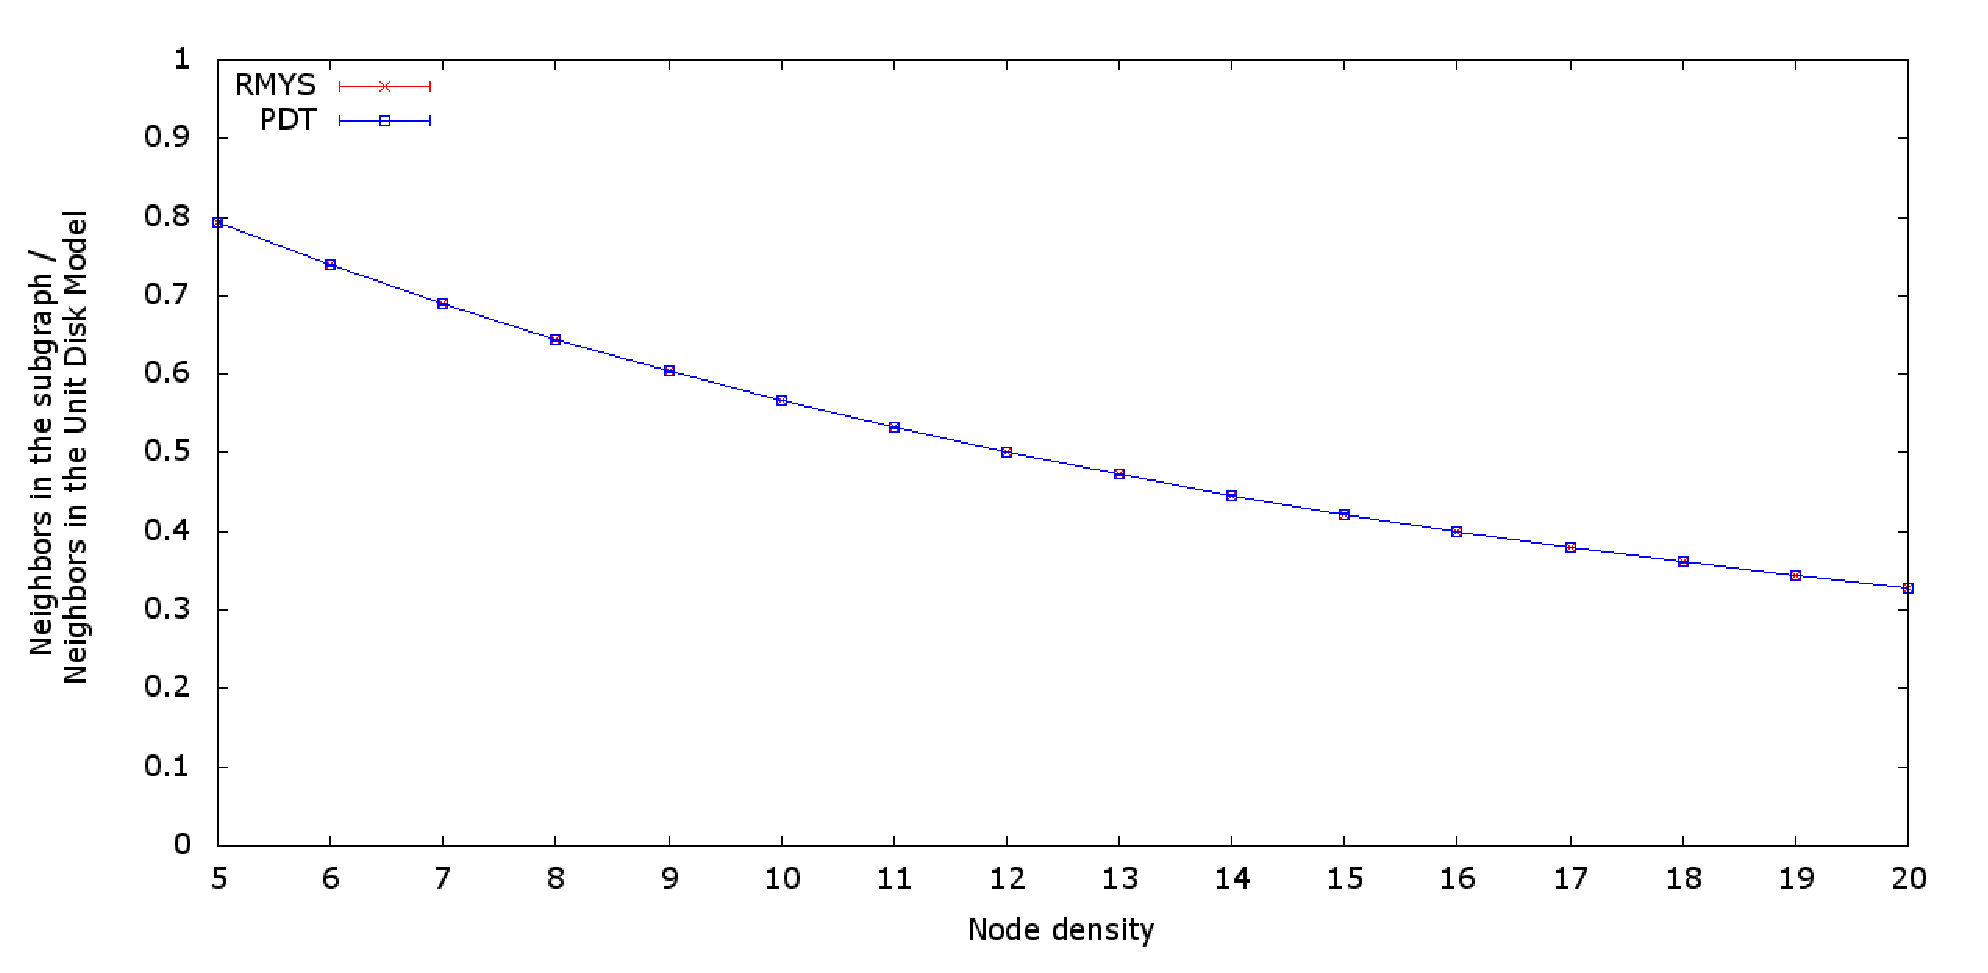
\includegraphics[width=1.0\linewidth]{RMYS_PDT_UDGNeighborsRatio.eps}
\end{frame}

\begin{frame}
\frametitle{Related work}
\begin{table}[h!]
\centering
\hspace*{-5mm}
\begin{tabular}{ccccc}
\hline 
Algorithm & Graph & Eucl. stretch & Max node degree & Ref. \\ 
\hline
BFP & GG & $\Theta{(\sqrt{n})} $ & $\mathcal{O}(n) $ & \cite{Ruhrup2010} \\ 

GDBF & GG & $\Theta{(\sqrt{n})} $ & $\mathcal{O}(n) $ & \cite{Chawla2006} \\ 

rPDT & PDT & $7.98 $ & $\mathcal{O}(n) $ & \cite{pdt, Neumann2012} \\ 

RMYS & S(PDT) & $\approx 7.98 $ \footnote{empirical proof} & 14 & my work \\
\hline 
\end{tabular} 
\label{table:topologies}
\end{table}
\end{frame}

\begin{frame}
\frametitle{Results}
RMYS:
\begin{itemize}
\item planar
\item constant node degree
\item reactive construction
\item connected graph
\item Euclidean t-spanner (empirical proof)
\end{itemize}
\end{frame}

\begin{frame}
\frametitle{Problem with spanner property}
\center for any connected unit disk graph $U $ the following is true:
\center $PDT(U) \subseteq UDEL(U) \subseteq LDEL^{(2)}(U) $
\end{frame}

\begin{frame}
\frametitle{Future work}
\begin{itemize}
\item formal proof that RMYS is indeed a spanner
\item consider reducing constant degree bound of $14 $ without increasing spanning ratio significantly.
\item consider reducing the message overhead when RMYS is executed on only one node
\end{itemize}
\end{frame}

\subsection{}
\begin{frame}
\center \Large Thanks for listening!
\center Do you have any questions?
\end{frame}


%ein Punkt p im roten Bereich sorgt dafür, dass u v auswählt als nächsten Nachbarn, v wählt jedoch p aus und nicht u. (uv kann trotzdem noch RMYS kannte sein, muss aber nicht, wenn alle anderen Cones voll sind.
\begin{frame}
	\frametitle{Non-bidirectional edge $uv$}
	\center 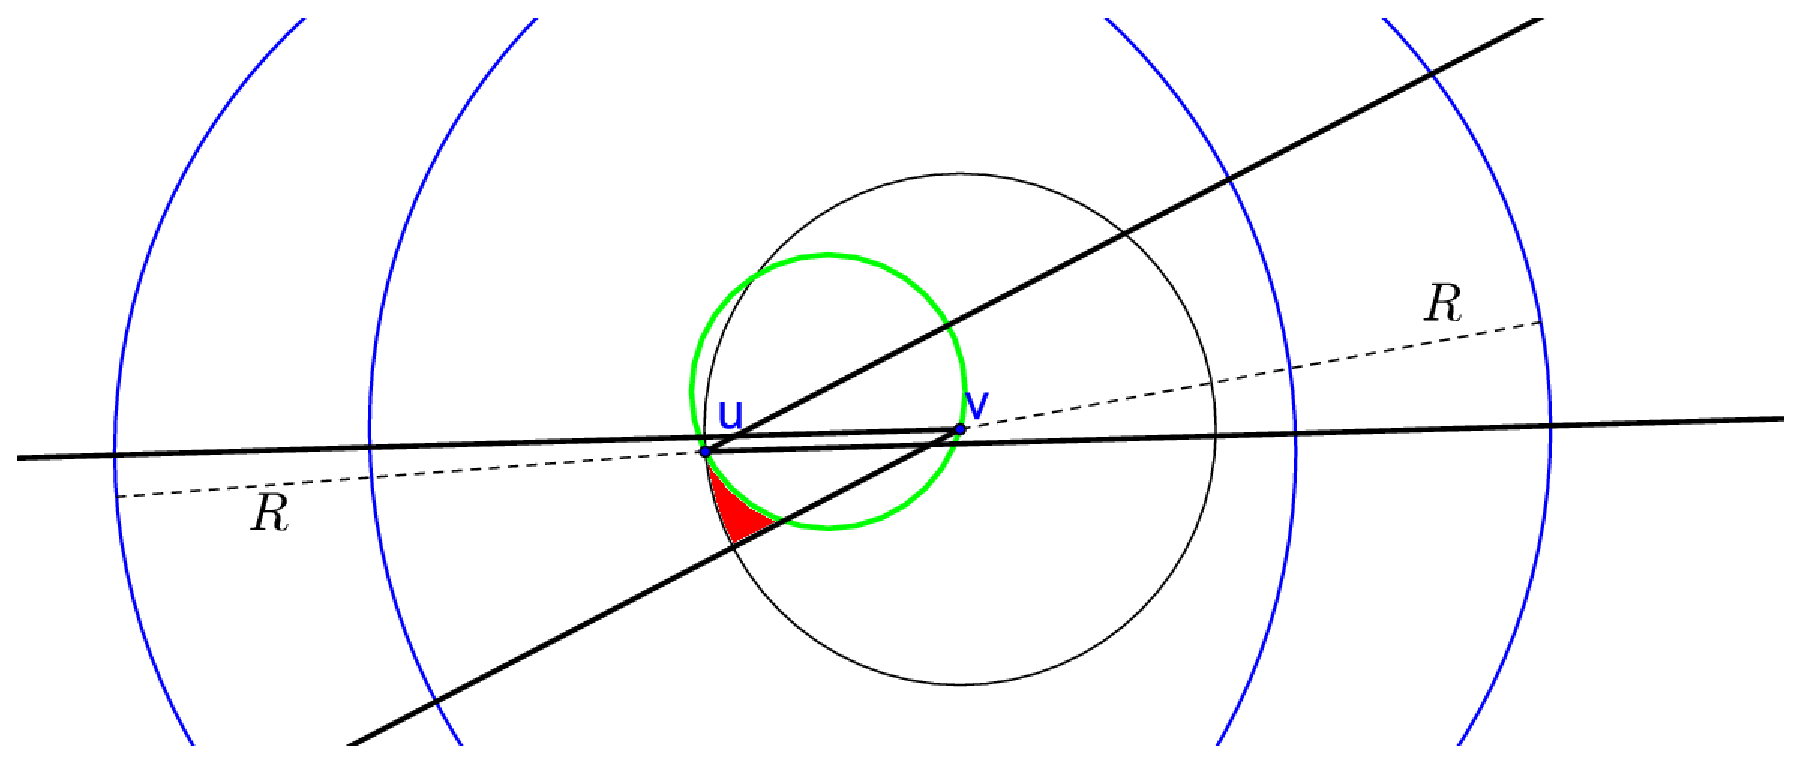
\includegraphics[width=1\linewidth]{RMYS_case_error_bidirectional.eps}
\end{frame}

%PDT Kante pv wird nicht ausgewählt, weil uv kürzeste ist und sonst keine sequence mit mehr als 1 leeren Cone existiert und beide angrenzenden cones nicht leer sind.
\begin{frame}
	\frametitle{PDT edge is not always a RMYS edge}
	\center 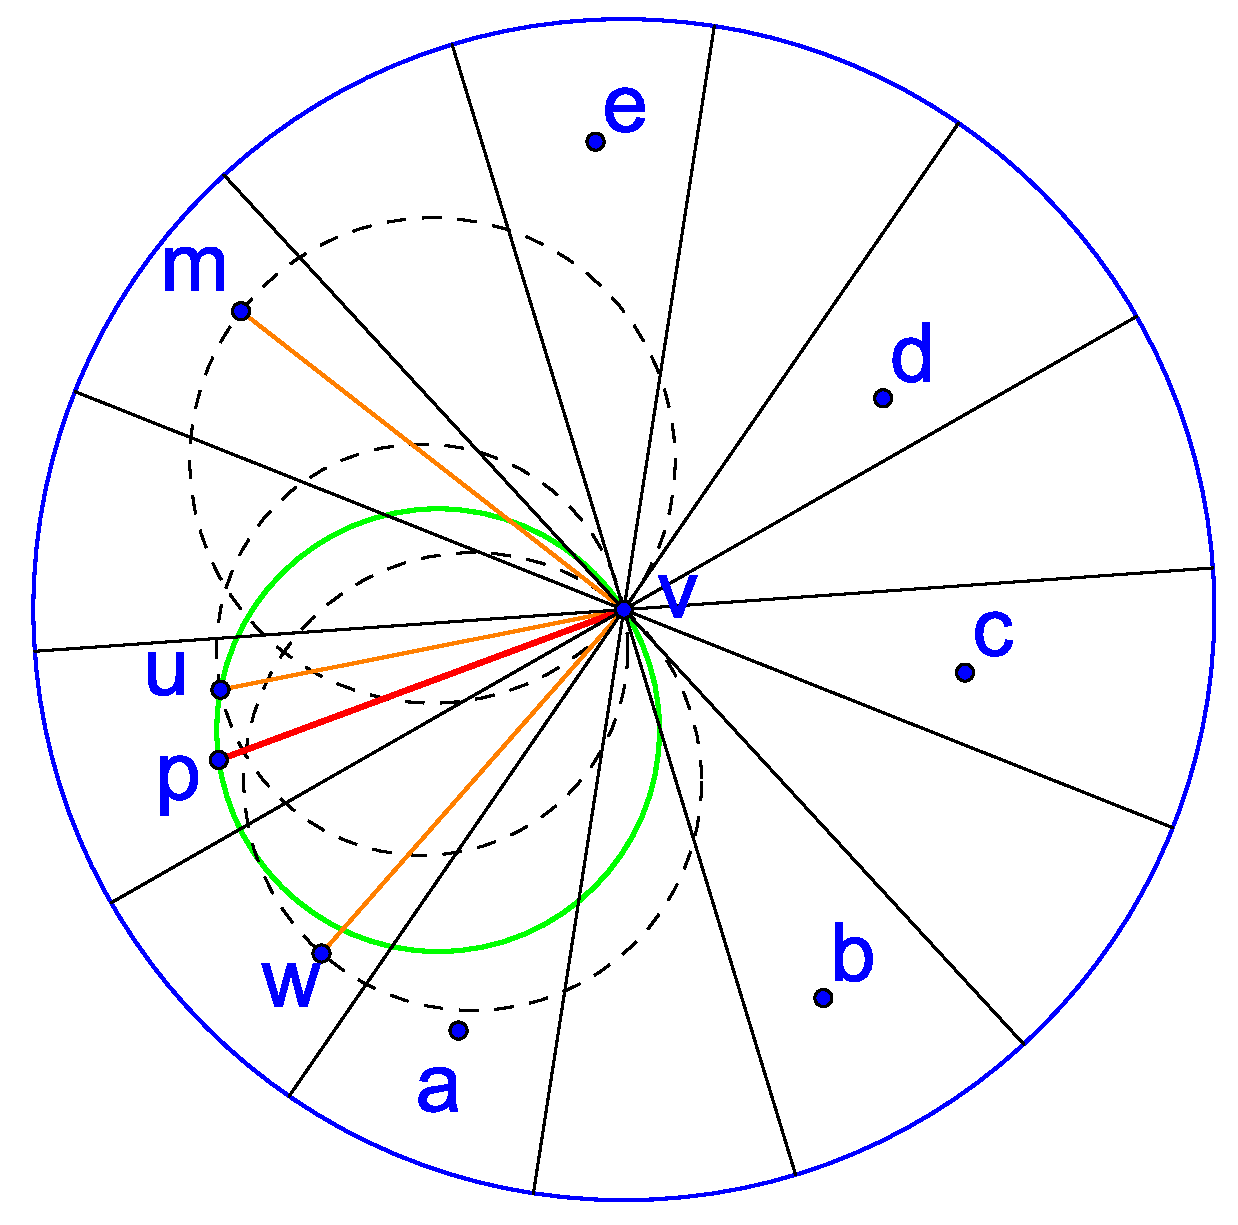
\includegraphics[width=0.7\linewidth]{RMYS_case_one_cone_empty.eps}
\end{frame}

\end{document}